\section{Sesión 4}

% En esta sesión estamos interesados en la evaluación de distintos mecanismos de reputación. Con este propósito,
% se ha utilizado una la configuración de entrenamiento DFL non-IID con la presencia de un nodo malicioso 
% realizando un \textit{flooding attack}. Sobre este escenario, se han usado dos configuraciones de reputación diferentes:

% \begin{itemize}
%     \item Reputación mediante \textit{pesos estáticos}.
%     \item Reputación mediante \textit{pesos dinámicos}.
% \end{itemize}

% En ambos casos, la reputación inicial de cada nodo se ha establecido en 0.5. Los pesos hacen referencia a la importancia
% relativa de cada métrica usada. En nuestro caso, usaremos siempre las 4 métricas disponibles, que se dividen en dos categorías:
% \textbf{métricas basadas en el modelo}, que incluyen \textit{Similitud del modelo} y \textit{Fracción de parámetros cambiados}, y
% \textbf{métricas basadas en la comunicación}, que incluyen \textit{Número de mensajes} y \textit{Latencia de llegada del modelo}.
% \vspace{1mm}

% En el caso del ataque de \textit{flooding}, el nodo malicioso trata de saturar la red. El sistema de reputación
% debe ser capaz de identificar este comportamiento anómalo y reducir la influencia del nodo atacante en el proceso
% de aprendizaje.

\subsection{Pesos estáticos}

% En esta configuración, se asignan pesos fijos a cada métrica para calcular la reputación de los nodos. Este método
% es muy sencillo pero poco flexible. Los pesos asignados son 0.30 / 0.15 / 0.30 / 0.25.

% \vspace{1mm}

Las reputaciones calculadas por cada nodo se muestran en la Figura \ref{fig:reputation_static}:

\vspace{1mm}
\noindent
\begin{minipage}{\textwidth}
    \centering
    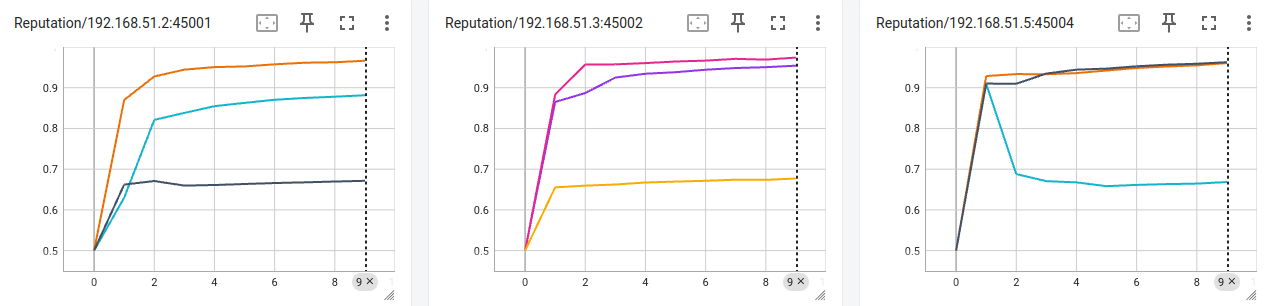
\includegraphics[width=0.9\textwidth]{images/reputation_static_rep.png}
    \captionof{figure}{Reputación con pesos estáticos a lo largo del entrenamiento.}
    \label{fig:reputation_static}
\end{minipage}
\vspace{1mm}

Vemos que los tres nodos honestos otorgan una reputación inferior al nodo malicioso.
Desde el punto de vista de cada nodo honesto, los demás nodos honestos tienen una
reputación muy cercana a 1, mientras que la reputación del nodo malicioso es algo
inferior a 0.7. Esta diferencia coincide con la poderación de la métrica de número
de mensajes (0.3), en la que el nodo malicioso obtiene una puntuación terrible (envía
alrededor de 15 mensajes por ronda). Dado que el nodo malicioso obtiene una buena puntuación
en las otras métricas, su reputación total se mantiene por encima de 0.5 y el nodo malicioso
se sigue considerando como honesto.

En cuanto a los resultados del entrenamiento con esta configuración, se muestran en la Figura \ref{fig:reputation_static_results}:
\vspace{1mm}

\begin{figure}[htbp]
    \centering
    % Primera imagen: f1
    \begin{minipage}{0.3\textwidth}
        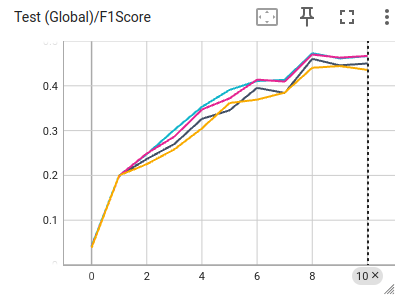
\includegraphics[width=\textwidth]{images/reputation_static_f1.png}
    \end{minipage}
    \hfill
    % Segunda imagen: cm
    \begin{minipage}{0.25\textwidth}
        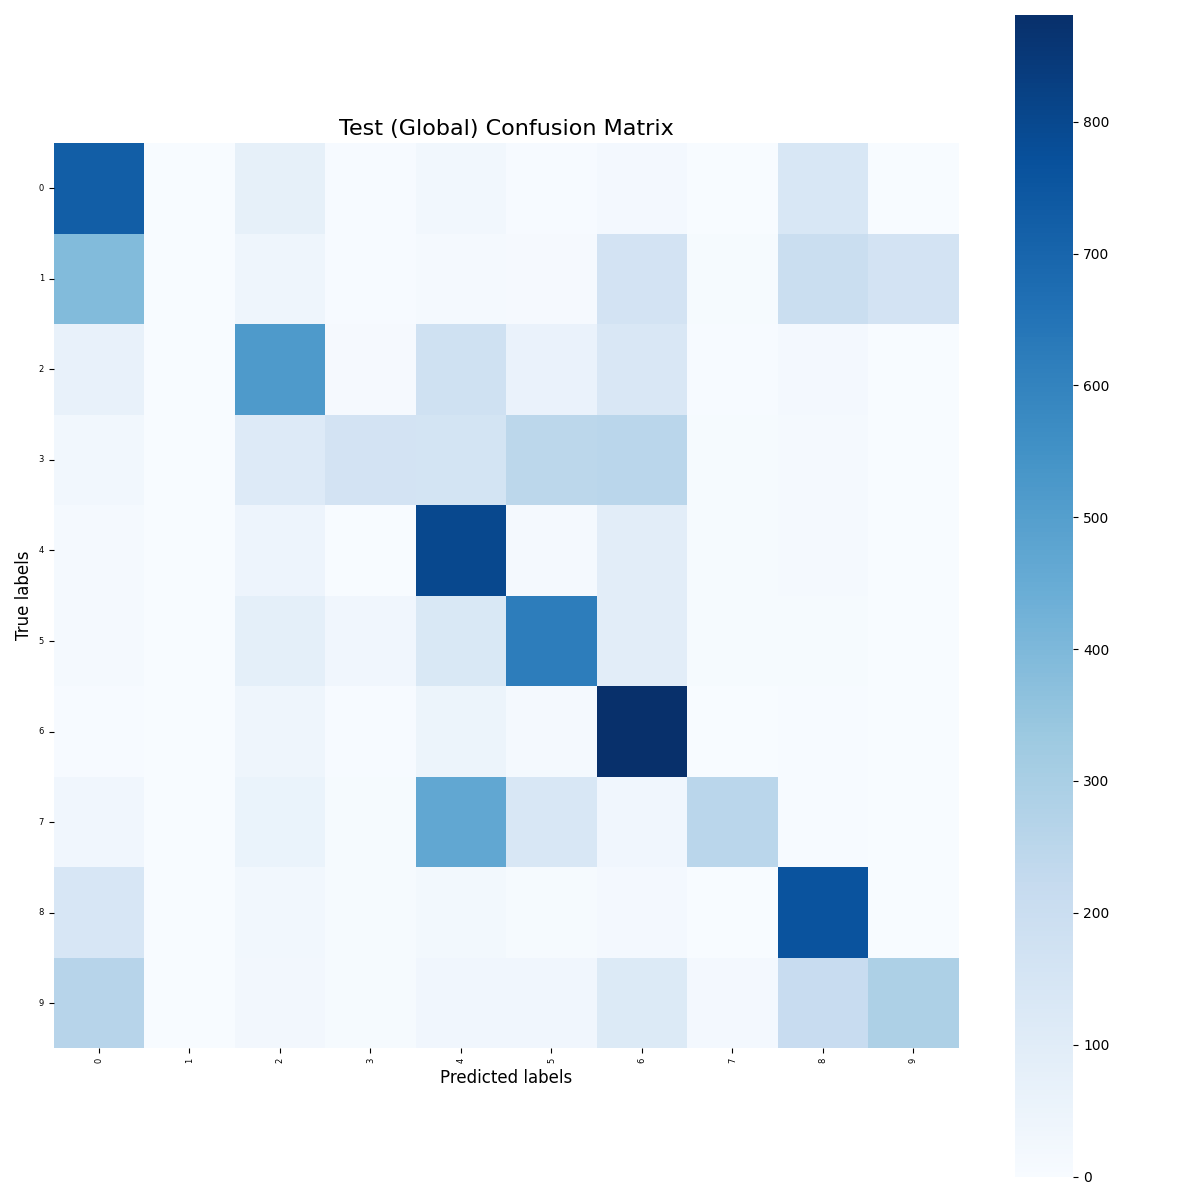
\includegraphics[width=\textwidth]{images/reputation_static_cm_honest.png}
    \end{minipage}
    \hfill
    % Tercera imagen: cm2
    \begin{minipage}{0.25\textwidth}
        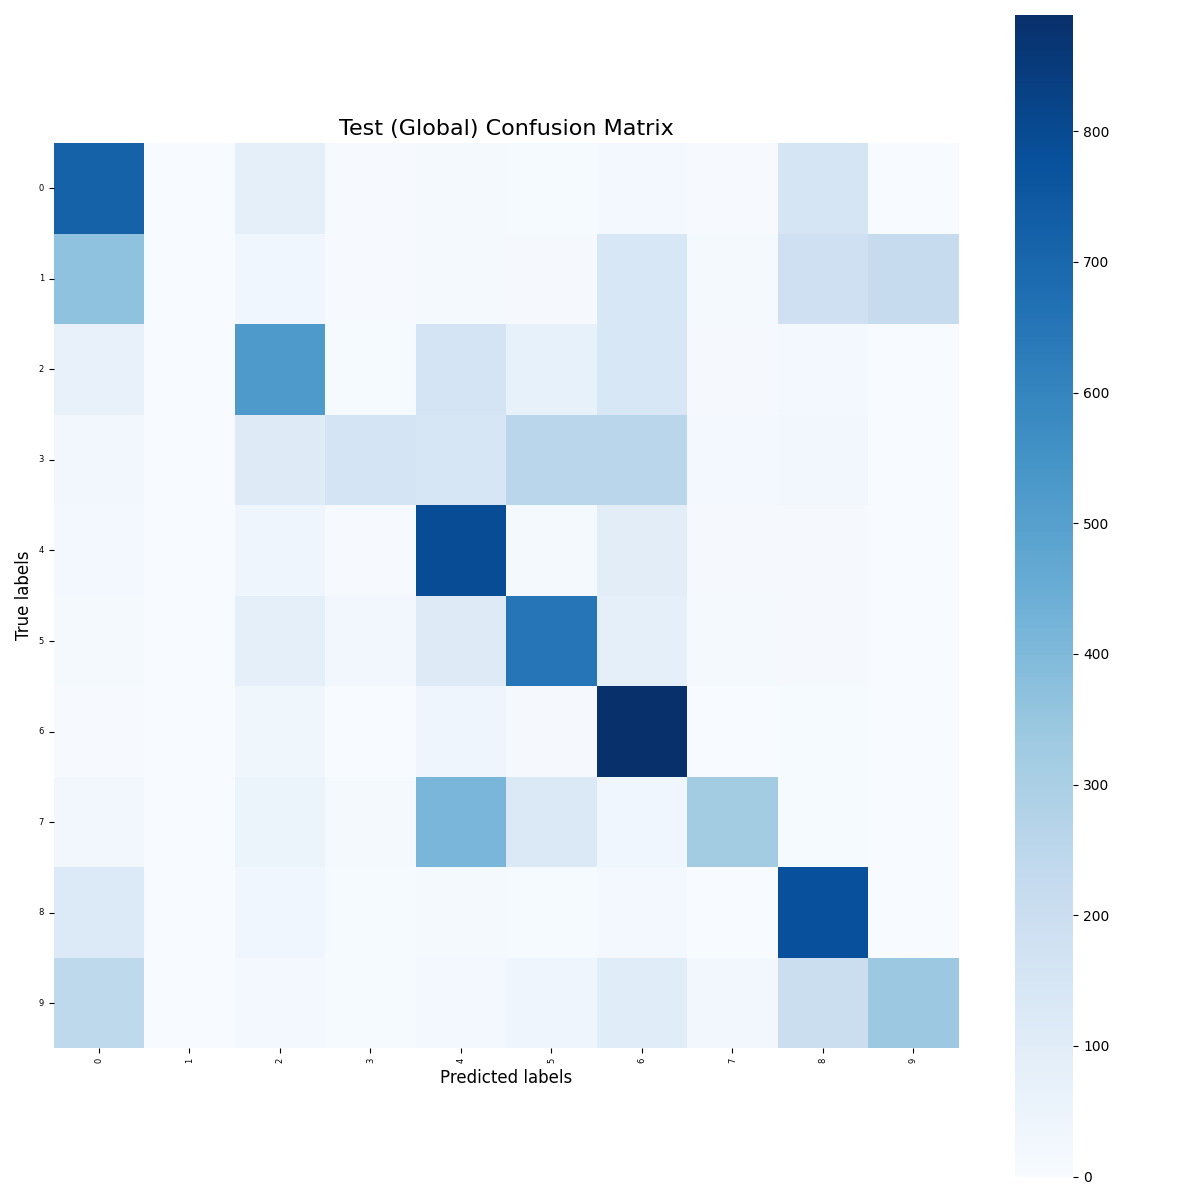
\includegraphics[width=\textwidth]{images/reputation_static_cm_malicious.png}
    \end{minipage}
    
    \caption{Resultados del entrenamiento con pesos estáticos: F1-score y matrices de confusión. Matriz de confusión del nodo malicioso a la derecha.}
    \label{fig:reputation_static_results}
\end{figure}

%REVISAR LA PRIMERA PARTE DE ESTE PÁRRAFO
La gráfica del F1-score apenas muestra señales del ataque. Los modelos alcanzan un F1-score cercano a 0.46,
mientras que el baseline (sin ataque) alcanza alrededor de 0.49. Esto es debido a que, a pesar del ataque 
de flooding, el contenido de los mensajes del nodo malicioso es correcto. El ataque resulta en un aumento del tráfico,
lo que si hace que el tiempo de entrenamiento esté cerca de duplicarse (4 minutos baseline vs 8 minutos con flooding y pesos estáticos).
Parte de este overhead puede ser debido también a la gestión de la reputación.
En cuanto a las matrices de confusión, las cuatro resultantes son prácticamente idénticas, lo que indica que los modelos han convergido.
A la izquierda se muestra la matriz de confusión de un nodo honesto y a la derecha la del nodo malicioso.

\subsection{Pesos dinámicos}

% En esta configuración, los pesos se ajustan dinámicamente para cada métrica en
% función de las condiciones del entorno.

% \vspace{1mm}

Los resultados se presentan en la Figura \ref{fig:reputation_dynamic}:

\vspace{1mm}
\noindent
\begin{minipage}{\textwidth}
    \centering
    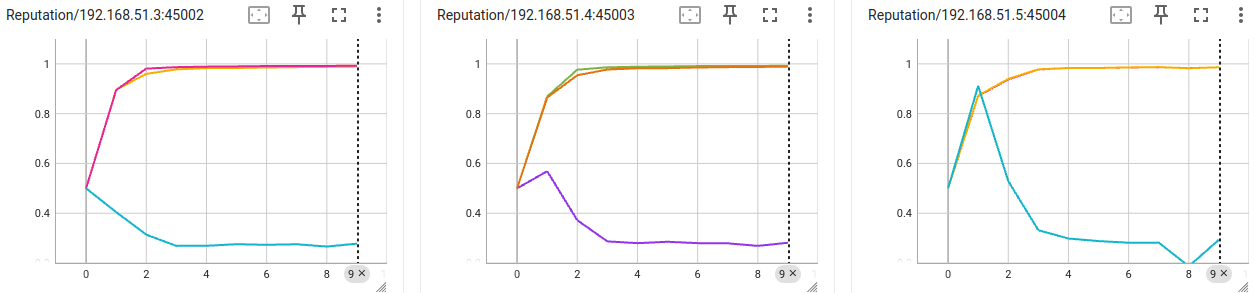
\includegraphics[width=0.9\textwidth]{images/reputation_dynamic_rep.png}
    \captionof{figure}{Reputación con pesos dinámicos a lo largo del entrenamiento.}
    \label{fig:reputation_dynamic}
\end{minipage}
\vspace{1mm}

En este caso, se observa que los nodos honestos asignan una reputación mucho más baja al nodo malicioso.
Esta vez la reputación del nodo malicioso cae hasta aproximadamente 0.3. Este valor, al quedar por debajo de 0.5, causa
la exclusión de las actualizaciones del nodo malicioso en el proceso de agregación. Sin embargo, parece que sí se le
siguen enviando las actualizaciones del modelo global, lo que permite que el nodo malicioso siga aprendiendo y mejorando
su rendimiento.
Los resultados del entrenamiento con esta configuración se muestran en la Figura \ref{fig:reputation_dynamic_results}:

\vspace{1mm}
\begin{figure}[htbp]
    \centering
    % Primera imagen: f1
    \begin{minipage}{0.3\textwidth}
        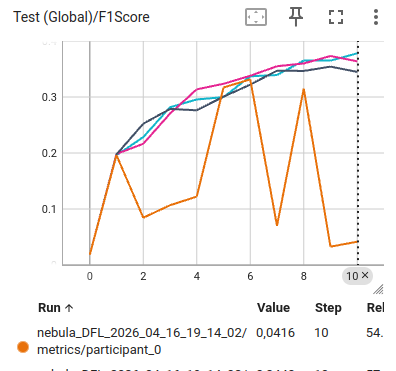
\includegraphics[width=\textwidth]{images/reputation_dynamic_f1.png}
    \end{minipage}
    \hfill
    % Segunda imagen: cm
    \begin{minipage}{0.25\textwidth}
        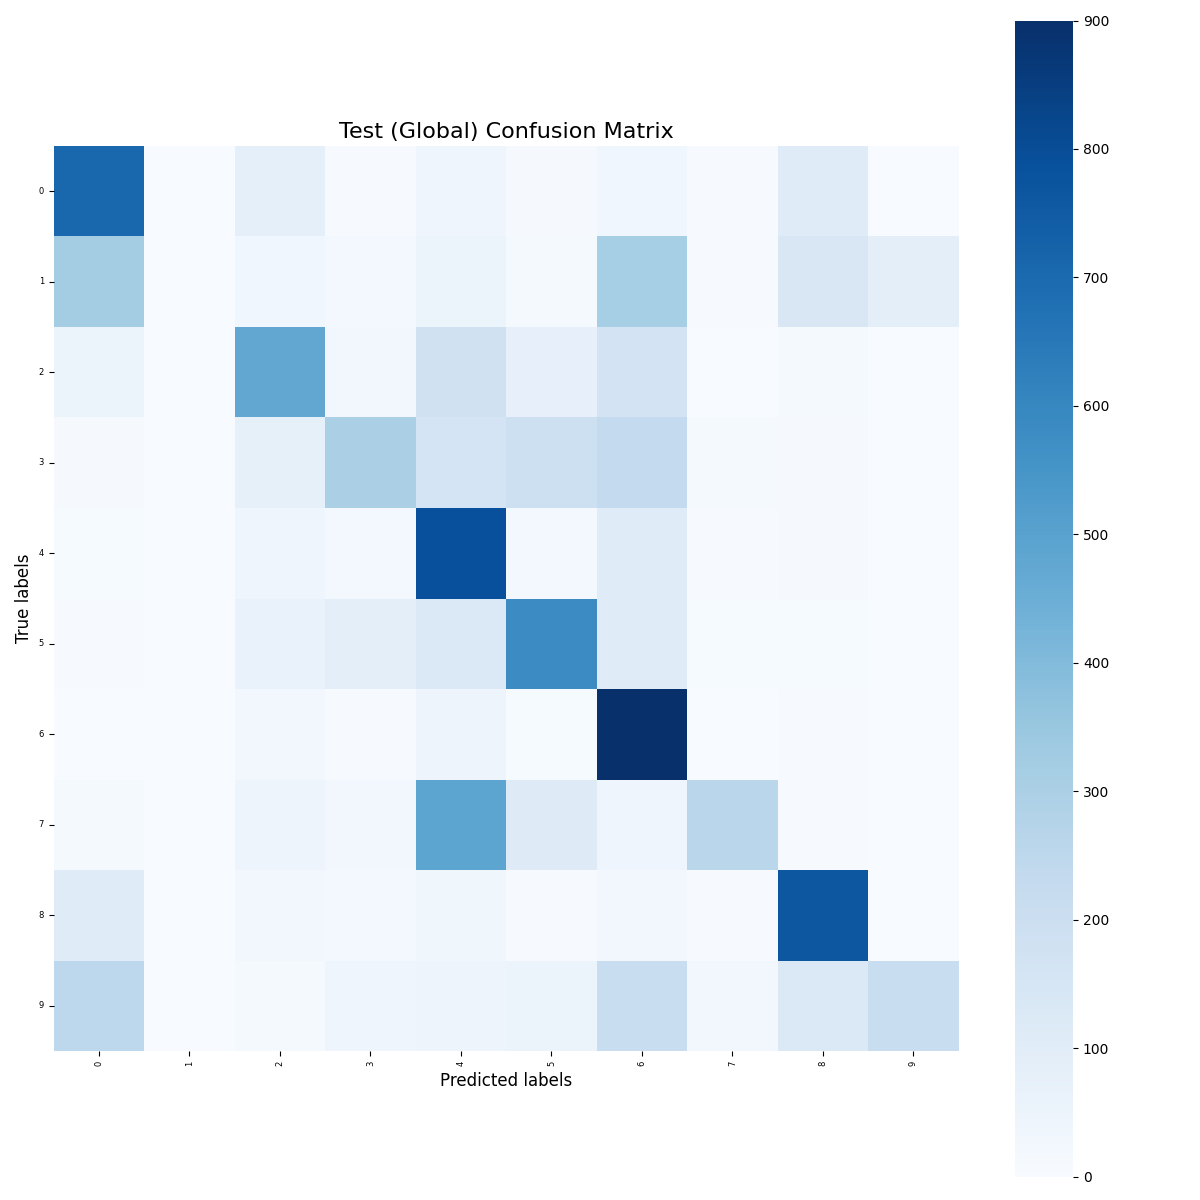
\includegraphics[width=\textwidth]{images/reputation_dynamic_honest_cm.png}
    \end{minipage}
    \hfill
    % Tercera imagen: cm2
    \begin{minipage}{0.25\textwidth}
        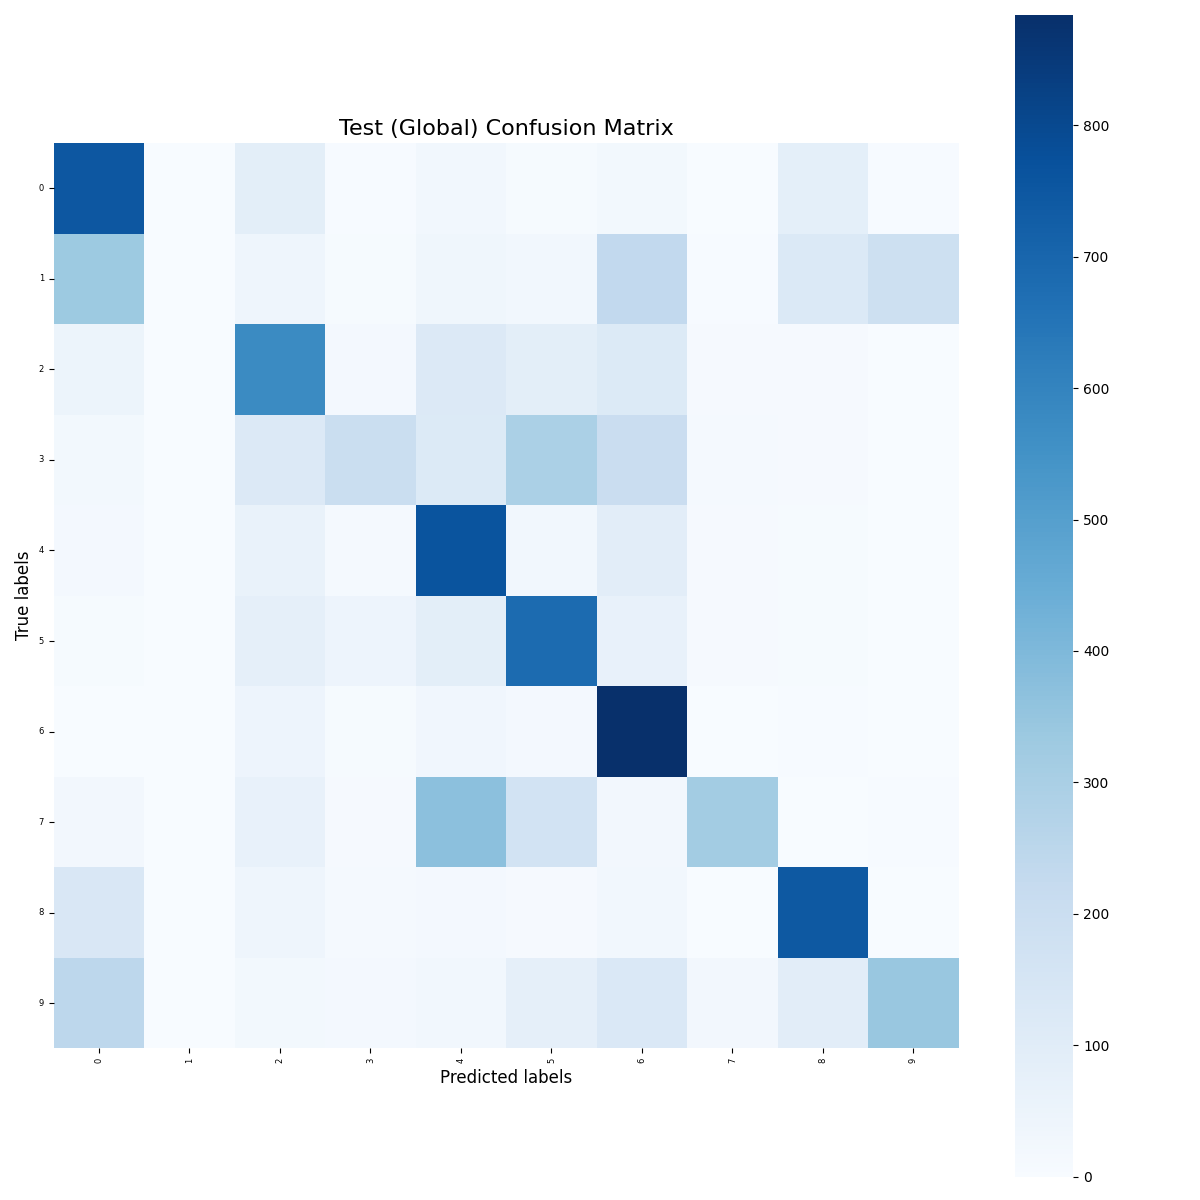
\includegraphics[width=\textwidth]{images/reputation_dynamic_malicious_cm.png}
    \end{minipage}
    
    \caption{Resultados del entrenamiento con pesos dinámicos: F1-score y matrices de confusión. Matriz de confusión del nodo malicioso a la derecha.}
    \label{fig:reputation_dynamic_results}
\end{figure}

La gráfica de F1-score es también similar a la anterior. Resulta curioso que el nodo malicioso obtenga un rendimiento
incluso mejor que el resto, lo que se debe a que es el único que sigue utilizando sus datos para entrenar (al tener
baja reputación, los otros nodos descartan sus actualizaciones). Esto, irónicamente, aporta cierta ventaja al nodo malicioso. El tiempo de
entrenamiento es muy similar al de la configuración de pesos estáticos. Esto puede ser debido a que el nodo malicioso
sigue enviando y recibiendo mensajes, aunque estos sean ignorados posteriormente.
En cuanto a las matrices de confusión, la de la izquierda es de un nodo honesto, mientras que la de la derecha corresponde
al nodo malicioso. De nuevo, los modelos convergen y las cuatro matrices de confusión son prácticamente idénticas.

\subsection{Comparación y análisis}

A partir de los resultados obtenidos, se pueden extraer las siguientes conclusiones:

\begin{itemize}
    \item La reputación con \textit{pesos dinámicos} demuestra una mayor capacidad de detección de ataques de \textit{flooding}, y cabe esperar que también sea superior a \textit{pesos estáticos} frente a otros tipos de ataques.
    \item Solo en el escenario con pesos dinámicos, el nodo malicioso es detectado y excluido completamente. Esta exclusión ocurre ya en la segunda ronda.
    \item La reacción de la federación ante el ataque es completamente ineficaz, incluso al detectarlo completamente. De hecho, la detección y exclusión de este causan que el modelo del
    atacante obtenga mejores resultados que los demás, cosa que no ocurriría si el ataque no fuera detectado.
\end{itemize}

%En conjunto, \textit{Trimmed Mean} resulta más adecuado en este escenario concreto, al ofrecer un mejor equilibrio entre robustez y estabilidad en presencia de nodos maliciosos y datos non-IID.

% ◼  Which configuration (static or dynamic) offered the best balance between robustness and 
% learning accuracy? 
% ◼  Did the reputation system detect and isolate malicious nodes early during training or from a 
% specific round?